% Set a pdf version and a document type
\ifx\pdfminorversion\undefined\else\pdfminorversion=4\fi
\documentclass[aspectratio=169,t,table]{beamer}

% Import all necessary packages
% Use this file to import all packages which are needed for the lecture
\usepackage[english]{babel}
\usepackage[utf8]{inputenc}
\usepackage[sfdefault]{roboto}
\usepackage[T1]{fontenc}
\usepackage{amsmath,amssymb}
\usepackage{graphicx}
\usepackage{listings}
\usepackage[backend=biber,sorting=none,doi=true,style=ieee]{biblatex}
\usepackage{url}
\usepackage{hyperref}
\usepackage{fontawesome5}
\usepackage{graphicx}
\usepackage{booktabs}
\usepackage{calc}
\usepackage{ifthen}
\usepackage{tabularx}
\usepackage{longtable}
\usepackage{makecell}
\usepackage{multicol}
\usepackage{multirow}
\usepackage{hhline}
\usepackage{qrcode}
\usepackage{xcolor}
\usepackage{cleveref}
\usepackage{tikz}
\usepackage{tikz-cd}
\usepackage{pgfplots,pgfplotstable,pgf-pie}
\usepackage[linesnumbered]{algorithm2e}
\usepackage{array}
\usepackage{mathtools}
\usepackage{verbatim}
\usetikzlibrary{patterns}
\usetikzlibrary{arrows.meta}


% Set the theme (customized FAU beamer theme)
\usetheme[%
	image,%
	longtitle,%
	inst=tf%
]{fau}

% Load the Git hash for the version
\input{x-additional/vc.tex}

% Set all important settings and define commands that are used in more than one lecture
% Set institute and date 
\institute[CS6]{Computer Science 6 (Data Management), Friedrich-Alexander-Universit\"at Erlangen-N\"urnberg}
\date[SS\the\year{}]{Summer semester \the\year{}}

% Configure the bibliography
\defbibheading{bibliography}{}
\addbibresource{references.bib}

% Define additional colors 
\definecolor{airforceblue}{rgb}{0.36, 0.54, 0.66}
\definecolor{ForestGreen}{rgb}{0.34, 0.139, 0.34}

% Configure the template
\setbeamercovered{transparent}
\setbeamertemplate{section in toc}[sections numbered]
\setbeamertemplate{section page}{%
	\begingroup
	\begin{beamercolorbox}[sep=10pt,center,rounded=true,shadow=true]{section title}
		\usebeamerfont{section title}\thesection~\insertsection\par
	\end{beamercolorbox}
	\endgroup
}
\setlength{\skip\footins}{0.2cm}
\setlength{\footnotesep}{0.1cm}

% Configure the formatting of listings
\lstset{%
	language=Python,
	tabsize=2,
	basicstyle=\tt,
	keywordstyle=\color{blue},
	commentstyle=\color{green!50!black},
	stringstyle=\color{red},
	numbers=left,
	numbersep=0.5em,
	xleftmargin=1em,
	numberstyle=\tt
}

% Add tikz and pgfplots libraries
\usetikzlibrary{arrows,decorations.pathmorphing,backgrounds,fit,positioning,shapes.symbols,chains,intersections,snakes,positioning,matrix,mindmap,shapes.multipart,shapes,calc,shapes.geometric,shadows,shadows.blur}
\usepgfplotslibrary{groupplots}

% Define pgfplotsset
\pgfplotsset{height=4cm,width=8cm,compat=1.14}

% Define tikz sets 
\tikzset{
	every overlay node/.style={
			anchor=north west, inner sep=0pt,
		},
}
\tikzset{
	thick,
	>=latex,
	every edge/.style={draw=gray, thick, >=latex},
	vertex/.style = {
			circle,
			fill            = black,
			outer sep = 2pt,
			inner sep = 1pt,
		}
}
\tikzset{level 1/.append style={sibling angle=50,level distance = 165mm}}
\tikzset{level 2/.append style={sibling angle=20,level distance = 45mm}}
\tikzset{every node/.append style={scale=1}}
\tikzset{
	vertex/.style = {
			circle,
			fill            = black,
			outer sep = 2pt,
			inner sep = 1pt,
		}
}
\tikzset{
	mynode/.style={
			draw,
			thick,
			anchor=south west,
			minimum width=2cm,
			minimum height=1.3cm,
			align=center,
			inner sep=0.2cm,
			outer sep=0,
			rectangle split,
			rectangle split parts=2,
			rectangle split draw splits=false},
	reverseclip/.style={
			insert path={(current page.north east) --
					(current page.south east) --
					(current page.south west) --
					(current page.north west) --
					(current page.north east)}
		}
}
\tikzset{basic/.style={
			draw,
			rectangle split,
			rectangle split parts=2,
			rectangle split part fill={blue!20,white},
			minimum width=2.5cm,
			text width=2cm,
			align=left,
			font=\itshape
		},
	Diamond/.style={ diamond,
			draw,
			shape aspect=2,
			inner sep = 2pt,
			text centered,
			fill=blue!10!white,
			font=\itshape
		}
}

% Define tikzoverlay
% Usage:
% \tikzoverlay at (-1cm,-5cm) {content};
% or
% \tikzoverlay[text width=5cm] at (-1cm,-5cm) {content};
\def\tikzoverlay{%
	\tikz[remember picture, overlay]\node[every overlay node]
}%

% Define additional math operators
\DeclareMathOperator*{\argmax}{arg\,max}
\DeclareMathOperator*{\argmin}{arg\,min}

% Define pgfmath functions
\pgfmathdeclarefunction{gauss}{2}{%
	\pgfmathparse{1/(#2*sqrt(2*pi))*exp(-((x-#1)^2)/(2*#2^2))}%
}

% Define additional commands
\newcommand*{\fullref}[1]{\underline{\hyperref[{#1}]{\cref{#1} (\nameref*{#1})}}}
\newcommand{\tikzmark}[1]{\tikz[remember picture] \node[coordinate] (#1) {#1};}
\newcommand{\plots}{0.611201}
\newcommand{\plotm}{2.19882}
\newcommand{\MaxNumberX}{3}
\newcommand{\MaxNumberY}{5}


% Title, author(s), and date
\title[KDDmUe~2.~Introduction]{2. Introduction} %
\subtitle{Knowledge Discovery in Databases with Exercises}
\author[D.~Probst]{Dominik Probst, \texttt{Dominik.probst@fau.de}}

% Metadata
\metadata{2. Introduction}{Introduction, Data Mining Process, Data Mining Challenges, Data Mining Applications, Interdisciplinary Context}{Introductory lecture on data mining/KDD: its purpose, process, challenges, applications, and interdisciplinary context.}

% Start the document
\begin{document}

% Title
\maketitle

{ % Outline
	\setbeamertemplate{footline}{}
	\begin{frame}[noframenumbering]{Outline}
		\tableofcontents

	\end{frame}
}

% Body
\section{Why data mining?}

\begin{frame}{Why Data Mining? (I)}
	\textbf{The explosive growth of data: from petabytes to exabytes to zettabytes\footnote{1 Zettabyte = 1,000,000,000,000,000,000,000 Byte (21 Zeros!)} and
		beyond.}\\
	\begin{itemize}
		\item Data collection and availability:
		      \begin{itemize}
			      \item Automated data collection tools.
			      \item Database systems.
			      \item World wide web.
			      \item Computerized society.
			      \item Digitization.
		      \end{itemize}
		\item Major sources of abundant data:
		      \begin{itemize}
			      \item Business: web, e-commerce, transactions, stocks \ldots
			      \item Science: remote sensing, bioinformatics, scientific
			            simulation \ldots
			      \item Society: news, digital cameras, social media \ldots
		      \end{itemize}
		\item The era of \textbf{big data} (as inflationary used buzzword).
	\end{itemize}
\end{frame}

\begin{frame}{Why Data Mining? (II)}
	\begin{figure}
		\centering
		\begin{tikzpicture}[scale=1]
			\begin{axis}[
					width=0.9\textwidth, height=0.7\textheight,
					ybar,
					symbolic x coords={2010,2011,2012,2013,2014,2015,2016,2017,2018,2019,2020,2021,2022,2023},
					xtick=data,
					xticklabel style={rotate=45, anchor=east},
					ymin=0,
					ymax=150,
					ylabel={Annual data volume generated \\ (in Zettabytes)\footnote{Source: \url{https://de.statista.com/statistik/daten/studie/267974/umfrage/prognose-zum-weltweit-generierten-datenvolumen/}}},
					ylabel style={align=center},
					xlabel={Year},
					enlargelimits=0.05,
					bar width=12pt,
					% nodes near coords,
					nodes near coords*={\pgfmathprintnumber{\pgfplotspointmeta}~ZB},
					every node near coord/.append style={font=\tiny},
					legend pos=north west,
				]
				\addplot[fill=gray!60] coordinates {(2010,2) (2011,5) (2012,6.5) (2013,9) (2014,12.5) (2015,15.5) (2016,18)
						(2017,26) (2018,33) (2019,41) (2020,64.2) (2021,84.5) (2022,103.66)
						(2023,132.4)};
			\end{axis}
		\end{tikzpicture}
	\end{figure}
\end{frame}

\begin{frame}{Why Data Mining? (III)}
	\textbf{The initial situation:}
	\begin{itemize}
		\item We are drowning in  data
		\item We are starving for knowledge
	\end{itemize}
	\textbf{The basic idea behind data mining:}
	\begin{itemize}
		\item We can analyze the data to satisfy our hunger for knowledge
	\end{itemize}
\end{frame}

\section{What is data mining?}

\begin{frame}{What is Data Mining?}
	\textbf{Data mining or knowledge discovery from data}:
	\begin{itemize}
		\item Extraction of interesting (\textbf{non-trivial, implicit,
			      previously unknown and potentially useful}) patterns from huge amounts
		      of data.
		\item Is \textbf{data mining} a misnomer?
	\end{itemize}
	Alternative names:
	\begin{itemize}
		\item Knowledge discovery/mining in databases (KDD).
		\item Knowledge extraction.
		\item Data/pattern analysis.
		\item Data archeology/dredging.
		\item Information harvesting.
		\item Business intelligence.
	\end{itemize}
\end{frame}

\begin{frame}{Examples: Is everything Data Mining?}
	Considered to be data mining:
	\begin{itemize}
		\item Analysis of customer behavior for user-related advertising.
		\item Analysis of payment histories for fraud detection.
		\item Analysis of infection behavior for better understanding of a
		      pandemic.
	\end{itemize}
	\textbf{NOT} considered to be data mining:
	\begin{itemize}
		\item Simple search for females in a customer database.
		\item Simple join of two database tables.
		\item Simple deductive database validating a new tuple with regards to
		      predefined constraints.
	\end{itemize}
\end{frame}

\begin{frame}{Data Mining in the Database-Systems Community}
	\begin{itemize}
		\item \textbf{Knowledge discovery pipeline} is a typical view from
		      the database-systems and data-warehousing community.
		\item Data mining plays an essential role in the knowledge-discovery
		      process.
	\end{itemize}
	\vspace{0.15cm}
	\centering
	\scalebox{0.95}{%
		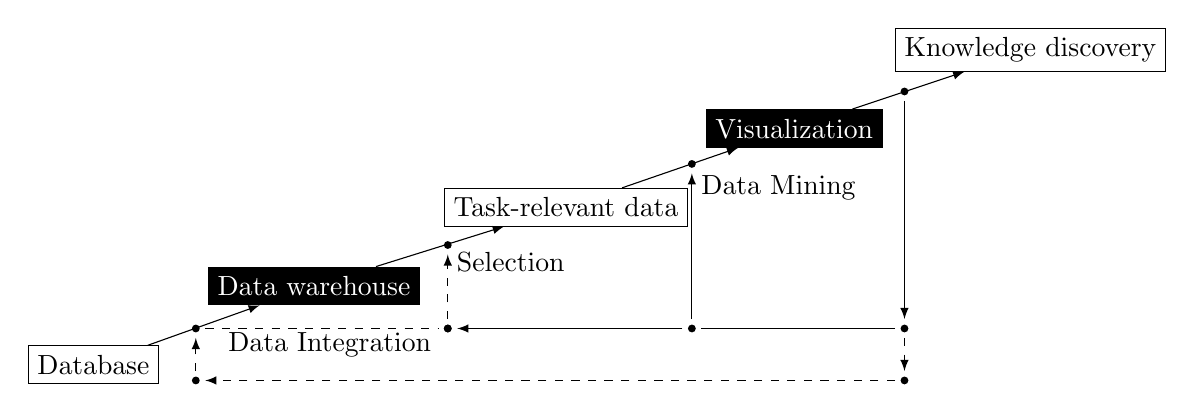
\begin{tikzpicture}
			% Dialectics
			\node[draw] (Database) at (0,0) {Database};
			\node[draw,fill=black,text=white] (Data warehouse) at (2.8,1) {Data
				warehouse};
			\node[draw] (Task-relevant data) at (6,2) {Task-relevant data};
			\node[draw,fill=black,text=white] (Data mining) at (8.9,3)
			{Visualization};
			\node[draw] (Knowledge discovery) at (11.9,4) {Knowledge discovery};

			\node (Data Integration) at (3,0.25) {Data Integration};
			\node (Selection) at (5.3,1.3) {Selection};
			\node (Data Mining) at (8.7,2.25) {Data Mining};

			\draw node[vertex] (Joint1) at (1.3,0.46) {};
			\draw node[vertex] (Joint2) at (4.5,1.52) {};

			\draw node[vertex] (Joint3) at (4.5,0.46) {};
			\draw node[vertex] (Joint7) at (4.5,0.46) {};
			\draw node[vertex] (Joint8) at (7.6,0.46) {};
			\draw node[vertex] (Joint9) at (10.3,0.46) {};
			\draw node[vertex] (Joint10) at (10.3,-0.2) {};
			\draw node[vertex] (Joint11) at (1.3,-0.2) {};

			\draw node[vertex] (Joint5) at (7.6,2.55) {};
			\draw node[vertex] (Joint6) at (10.3,3.47) {};


			\draw[->,draw=black] (Database) to (Data warehouse);
			\draw[->,draw=black] (Data warehouse) to (Task-relevant data);
			\draw[->,draw=black] (Task-relevant data) to (Data mining);
			\draw[->,draw=black] (Data mining) to (Knowledge discovery);
			\draw[-,draw=black, dashed] (Joint1) to (Joint3);
			\draw[->,draw=black, dashed] (Joint3) to (Joint2);
			\draw[->,draw=black] (Joint6) to (Joint9);
			\draw[-,draw=black] (Joint9) to (Joint8);
			\draw[->,draw=black] (Joint8) to (Joint7);
			\draw[->,draw=black] (Joint8) to (Joint5);
			\draw[->,draw=black,dashed] (Joint10) to (Joint11);
			\draw[->,draw=black,dashed] (Joint9) to (Joint10);
			\draw[->,draw=black,dashed] (Joint11) to (Joint1);
		\end{tikzpicture}
	}
\end{frame}

\begin{frame}{Data Mining in the Business Community}
	\centering
	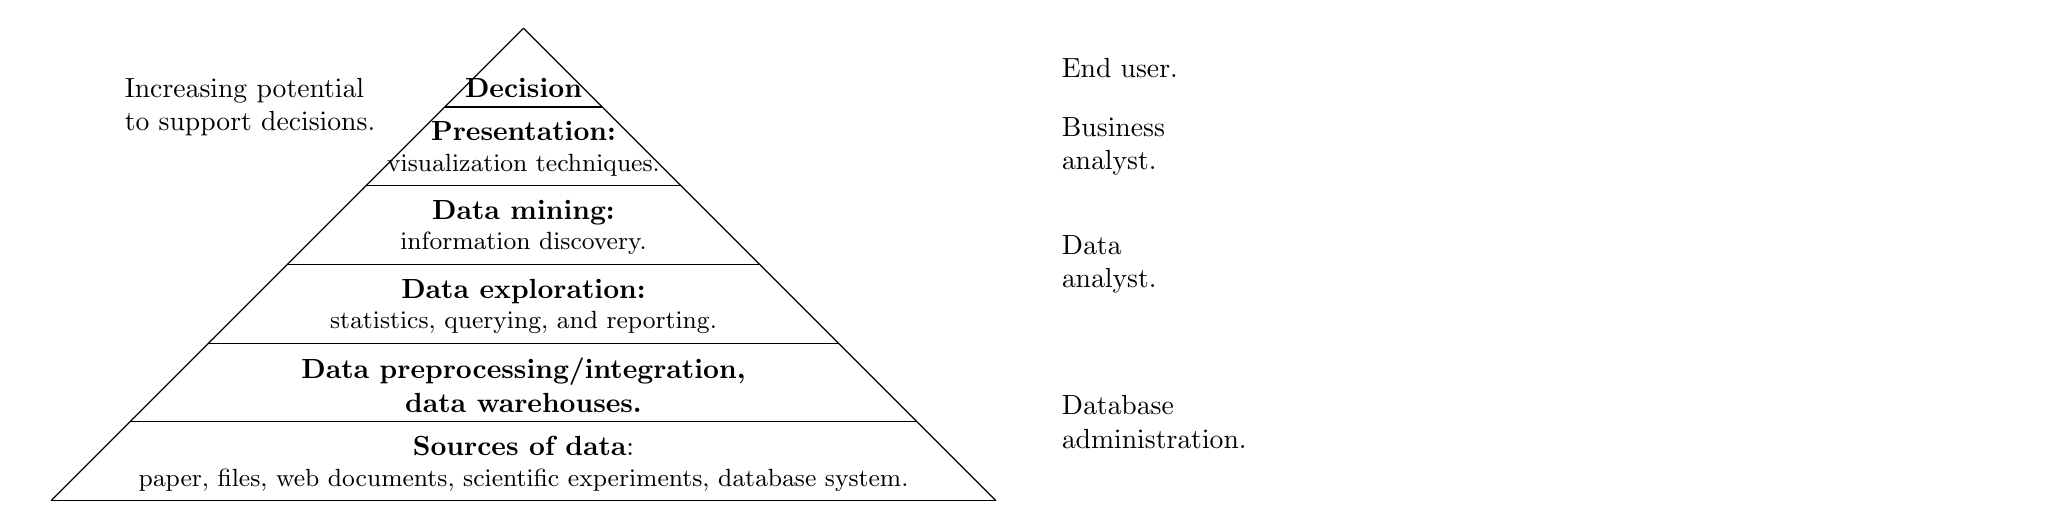
\begin{tikzpicture}
		\coordinate (A) at (-6,0) {};
		\coordinate (B) at ( 6,0) {};
		\coordinate (C) at (0,6) {};
		\draw[name path=AC] (A) -- (C);
		\draw[name path=BC] (B) -- (C);

		\node (Data Integration) at (1,5) {\parbox{\linewidth}{Increasing
				potential \\ to support decisions.}};
		\node (Data Integration) at (12.9,1) {\parbox{\linewidth}{Database \\
				administration.}};
		\node (Data Integration) at (12.9,3) {\parbox{\linewidth}{Data \\
				analyst.}};
		\node (Data Integration) at (12.9,4.5) {\parbox{\linewidth}{Business \\
				analyst.}};
		\node (Data Integration) at (12.9,5.5) {\parbox{\linewidth}{End user.}};

		\foreach \y/\A in {
		0/{
		\parbox{\linewidth}{
			\centering
			\textbf{Sources of data}: \\
			\small{paper, files, web documents, scientific experiments,
				database system.}}
		},
		1/{
		\parbox{\linewidth}{
			\centering
			\textbf{Data preprocessing/integration,\\
				data warehouses.}}
		},
		2/{
		\parbox{\linewidth}{
			\centering
			\textbf{Data exploration:} \\
			\small{statistics, querying, and reporting.}}
		},
		3/{
		\parbox{\linewidth}{
			\centering
			\textbf{Data mining:} \\
			\small{information discovery.}}
		},
		4/{
		\parbox{\linewidth}{
			\centering
			\textbf{Presentation:} \\
			\small{visualization techniques.}}
		},
		5/{
		\parbox{\linewidth}{
			\centering
			\textbf{Decision}}
		}
		} {
		\path[name path=horiz] (A|-0,\y) -- (B|-0,\y);
		\draw[name intersections={of=AC and horiz,by=P},
			name intersections={of=BC and horiz,by=Q}] (P) -- (Q)
		node[midway,above] {\A};
		}
	\end{tikzpicture}
\end{frame}

\begin{frame}{Data Mining in the Machine Learning and Statistics Community}
	Machine-learning and statistics communities usually classify data mining as
	the central part of their pipeline:

	\vspace{0.5cm}
	\centering
	\scalebox{0.95}{%
		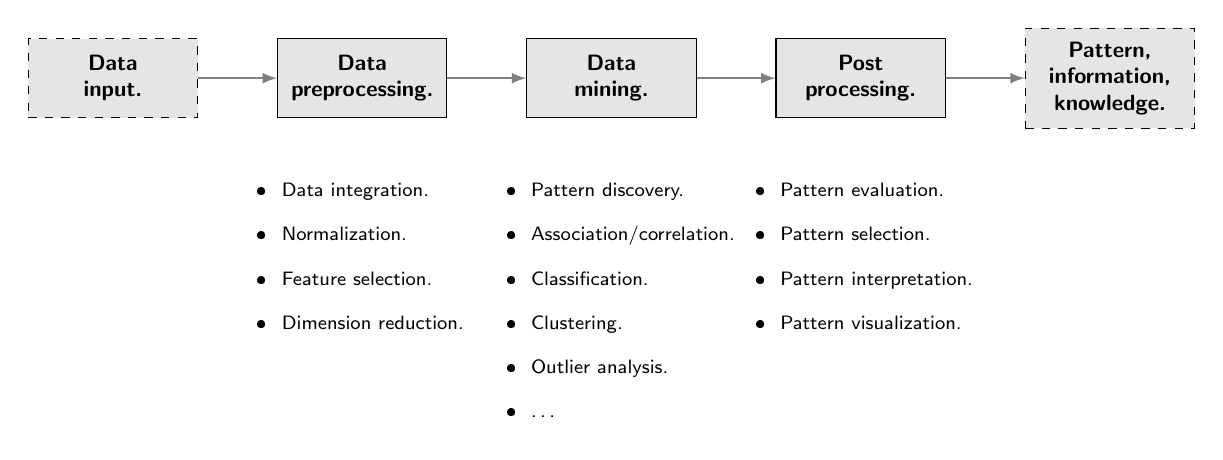
\begin{tikzpicture}
			[node distance = 1cm, auto,font=\footnotesize,
				% STYLES
				every node/.style={node distance=1cm},
				% The comment style is used to describe the characteristics of each
				%force
				comment/.style={rectangle, inner sep= 5pt, text width=3.8cm, node
						distance=0.5cm, font=\scriptsize\sffamily},
				% The force style is used to draw the forces' name
				force/.style={rectangle, draw, fill=black!10, inner sep=5pt, text
						width=1.8cm, text badly centered, minimum height=1cm,
						font=\bfseries\footnotesize\sffamily}]

			% Draw forces
			\node [force, dashed] (a) {\parbox{\linewidth}{\centering Data \\
					input.}};
			\node [force, right=1cm of a] (b) {\parbox{\linewidth}{\centering
					Data
					\\ preprocessing.}};
			\node [force, right=1cm of b] (c) {\parbox{\linewidth}{\centering
					Data
					\\ mining.}};
			\node [force, right=1cm of c] (d) {\parbox{\linewidth}{\centering
					Post
					\\ processing.}};
			\node [force, dashed, right=1cm of d] (e)
			{\parbox{\linewidth}{\centering Pattern, \\ information, \\
					knowledge.}};

			%%%%%%%%%%%%%%%
			% Change data from here

			% SUPPLIERS
			\node [comment, below=0.25cm of b] {
				\begin{itemize}
					\item Data integration.
					\item Normalization.
					\item Feature selection.
					\item Dimension reduction.
				\end{itemize}
			};

			% USERS
			\node [comment, below=0.25 of c] {
				\begin{itemize}
					\item Pattern discovery.
					\item Association/correlation.
					\item Classification.
					\item Clustering.
					\item Outlier analysis.
					\item \ldots
				\end{itemize}
			};

			% PUBLIC POLICIES
			\node [comment, below=0.25 of d] {
				\begin{itemize}
					\item Pattern evaluation.
					\item Pattern selection.
					\item Pattern interpretation.
					\item Pattern visualization.
				\end{itemize}
			};

			\path[->,thick]
			(a) edge (b)
			(b) edge (c)
			(c) edge (d)
			(d) edge (e);

		\end{tikzpicture}
	}
\end{frame}

\begin{frame}{The Data Mining Process: CRISP-DM}
	\begin{itemize}
		\item \textbf{CRoss-Industry Standard Process for Data Mining}:
	\end{itemize}
	\vspace{0.5cm}
	\centering
	\scalebox{0.95}{%
		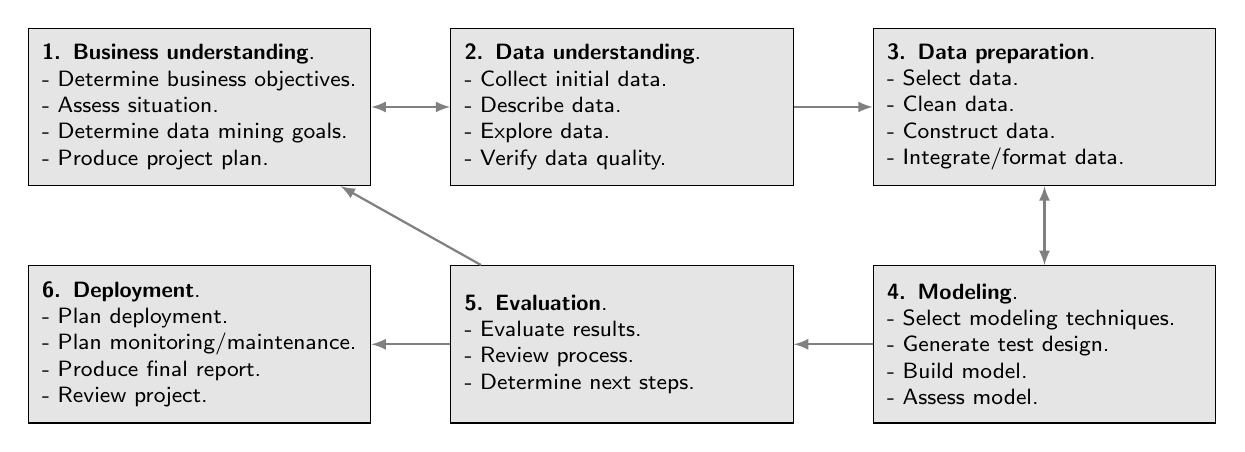
\begin{tikzpicture}
			[node distance = 2cm, auto,font=\footnotesize,
				% STYLES
				every node/.style={node distance=2cm},
				% The comment style is used to describe the characteristics of each
				%force
				comment/.style={rectangle, inner sep= 5pt, text width=5cm, node
						distance=0.5cm, font=\scriptsize\sffamily},
				% The force style is used to draw the forces' name
				force/.style={rectangle, draw, fill=black!10, inner sep=5pt, text
						width=4cm, minimum height=2cm, font=\footnotesize\sffamily}]

			% Draw forces
			\node [force] (a) {
				\parbox{\linewidth}{
					\textbf{1. Business understanding}.\\
					- Determine business objectives.\\
					- Assess situation.\\
					- Determine data mining goals.\\
					- Produce project plan.
				}
			};
			\node [force, right=1cm of a] (b) {
				\parbox{\linewidth}{
					\textbf{2. Data understanding}.\\
					- Collect initial data.\\
					- Describe data.\\
					- Explore data.\\
					- Verify data quality.
				}
			};
			\node [force, right=1cm of b] (c) {
				\parbox{\linewidth}{
					\textbf{3. Data preparation}.\\
					- Select data.\\
					- Clean data.\\
					- Construct data.\\
					- Integrate/format data.
				}
			};
			\node [force, below=1cm of c] (d) {
				\parbox{\linewidth}{
					\textbf{4. Modeling}.\\
					- Select modeling techniques.\\
					- Generate test design.\\
					- Build model.\\
					- Assess model.
				}
			};
			\node [force, below=1cm of a] (e) {
				\parbox{\linewidth}{
					\textbf{6. Deployment}.\\
					- Plan deployment.\\
					- Plan monitoring/maintenance.\\
					- Produce final report.\\
					- Review project.
				}
			};
			\node [force, below=1cm of b] (f) {
				\parbox{\linewidth}{
					\textbf{5. Evaluation}.\\
					- Evaluate results.\\
					- Review process.\\
					- Determine next steps.
				}
			};

			\path[->,thick]
			(b) edge (c)
			(d) edge (f)
			(f) edge (e)
			(f) edge (a);

			\path[<->,thick]
			(a) edge (b)
			(c) edge (d);
		\end{tikzpicture}
	}
\end{frame}

\section{A Multidimensional View of Data-Mining}

\begin{frame}{A Multidimensional View of Data Mining}
	\textbf{Data mining projects can be described in four dimensions:}
	\begin{itemize}
		\item \textbf{What data is available?}:\\
		      \small{
			      Data can exist in a wide variety of forms and must therefore be
			      treated differently in data mining.
		      }
		\item \textbf{What patterns are searched for?}:\\
		      \small{
			      Various functions in data mining can be used to detect
			      different patterns.
		      }
		\item \textbf{What technologies are used?}:\\
		      \small{
			      The technologies used can vary greatly in data mining.
		      }
		\item \textbf{What is the actual target application?}:\\
		      \small{
			      The actual target application also differs from case to case.
		      }
	\end{itemize}
\end{frame}

\section{What kind of data can be mined?}

\begin{frame}{What kind of data can be mined?}
	\begin{itemize}
		\item Database oriented data sets and applications:
		\begin{itemize}
			\item Relational database.
			\item Data warehouse.
			\item Transactional database.
		\end{itemize}
		\item Advanced data sets and advanced applications:
		\begin{itemize}
			\item Data streams and sensor data.
			\item Time series data, temporal data, sequence data (incl. 
			biosequences).
			\item Structure data, graphs, social networks and multi-linked data.
			\item Object-relational databases.
			\item Heterogeneous databases and legacy databases.
			\item NoSQL databases.
			\item Spatial data and spatiotemporal data.
			\item Multimedia databases.
		\end{itemize}
	\end{itemize}
\end{frame}
\section{What kind of patterns can be mined?}

\begin{frame}{What kind of patterns can be mined?}
	\begin{itemize}
		\item \textbf{Searching for the right patterns is important.}
		\item Which patterns can be mined depends on:
		\begin{itemize}
			\item \textbf{The data mining function} \\
				  \small{Different functions can reveal different patterns.}
			\item \textbf{The data set} \\
				  \small{Some types of records contain special patterns that 
				  can be found only in them.}
		\end{itemize}
		\item Patterns do not always lead to useful information. \\
				$\rightarrow$ Always validate whether the gained knowledge is 
				interesting
	\end{itemize}
\end{frame}

\begin{frame}{Data Mining Function: I. Generalization}
	\textbf{Information integration and data warehouse construction:}
	\begin{itemize}
		\item Data cleaning.
		\item Transformation.
		\item Integration.
		\item Multidimensional modeling.
	\end{itemize}
	\textbf{Data cube technology:}
	\begin{itemize}
		\item Characterization (contrast data characteristics).\\
		E.g. dry vs. wet regions from numerical humidity values.
		\item Discrimination.
		\item Generalization.
		\item Summary.
	\end{itemize}
\end{frame}

\begin{frame}{Data Mining Function: II. Association and Correlation Analysis}
	\textbf{Frequent patterns or item sets:}\\
	What items are frequently purchased together in your supermarket.\\[0.5cm]
	
	\textbf{Association, correlation vs. causality:}\\
	A typical association rule: Diapers $\rightarrow$ Beer $[0.5\%,75\%]$ 
	(support, confidence).\\
	Are strongly associated items also strongly correlated?\\[0.5cm]
	
	\textbf{How to mine such patterns and rules efficiently in large 
	datasets?}\\
	\textbf{How to use such patterns for classification, clustering and other 
	applications?}
\end{frame}

\begin{frame}{Data Mining Function: III. Classification}
	\textbf{Classification and (class-)label prediction:}\\
	Construct models (functions) based on training examples. \\
	Hence: "supervised".\\
	Describe and distinguish classes or concepts for future prediction.\\
	E.g. classify countries based on climate or classify cars based on gas 
	mileage.\\
	Classifying something means to predict unknown class labels. \\[0.5cm]
	
	\textbf{Typical methods:}\\
	Decision trees, naive Bayesian classification, support-vector machines, 
	neural networks, rule-based classification, pattern-based classification, 
	logistic regression \ldots\\[0.5cm]
	
	\textbf{Typical applications:}\\
	Credit-card-fraud detection, direct marketing, classifying stars, diseases, 
	web pages \ldots
\end{frame}

\begin{frame}{Data Mining Function: IV. Cluster Analysis}
	\textbf{Unsupervised learning:} I.e. class labels are unknown.\\
	\textbf{Group data:} I.e. cluster houses to find distribution 
	patterns.\\[0.5cm]
	
	Principle:\\
	Maximize intra class similarity and minimize inter class 
	similarity.\\[0.5cm]
	
	What is \textbf{similarity?}
\end{frame}

\begin{frame}{Data Mining Function: V. Outlier Analysis}
	\textbf{Outlier}: A data object that does not comply with the general 
	behavior of the data.\\[0.5cm]
	
	Noise or exception?\\
	One person's garbage could be another person's treasure.\\[0.5cm]
	
	\textbf{Methods:}\\
	By-product of clustering or regression analysis \ldots \\
	Useful in fraud detection or rare-events analysis.
\end{frame}

\begin{frame}{Time and Ordering: Sequential Pattern, Trend and Evolution 
Analysis}
	\textbf{Sequence, trend, and evolution analysis}.\\
	\begin{itemize}
		\item Trend, time-series and deviation analysis. \\
		E.g., regression and value prediction (forecasting).
		\item Sequential-pattern mining.\\
		E.g. customers first buy a digital camera, then buy large SD memory 
		cards.
		\item Periodicity analysis.
		\item Motifs and biological-sequence analysis.\\
		Approximate and consecutive motifs.
		\item Similarity-based analysis.\\
		\item Mining data streams.\\
		Ordered, time-varying, potentially infinite (unbounded).
	\end{itemize}
\end{frame}

\begin{frame}{Structure and Network Analysis}
	\textbf{Graph mining}:\\
	Finding frequent subgraphs (e.g. chemical compounds), trees (XML), 
	substructures (web fragments), information-network analysis.\\[0.2cm]
	
	\textbf{Social networks}:
	\begin{itemize}
		\item Social networks: Actors (objects, nodes) and relationships 
		(edges).\\
		E.g., author networks in CS, terrorist networks.
		\item Multiple heterogeneous networks.\\
		A person could be in multiple information networks: friends, family, 
		classmates \ldots
		\item Links carry a lot of semantical information: link mining.
	\end{itemize}
	
	\textbf{Web mining}:
	\begin{itemize}
		\item Web is a big information network: from PageRank to Google.
		\item Analysis of web information networks.
		\item Web community discovery, opinion mining, usage mining \ldots
	\end{itemize}
\end{frame}

\begin{frame}{Evaluation of Knowledge}
	\textbf{Is all mined knowledge interesting?}
	\begin{itemize}
		\item One can mine tremendous amounts of "patterns" and knowledge.
		\item Some may fit only certain dimension space (time, location \ldots).
		\item Some may not be representative, may be transient \ldots
	\end{itemize}
	
	\textbf{Evaluation of mined knowledge $\rightarrow$ directly mine only 
	interesting knowledge?}
	\begin{itemize}
		\item Descriptive vs. predictive.
		\item Coverage.
		\item Typically vs. predictive.
		\item Accuracy.
		\item Timeliness.
		\item \ldots
	\end{itemize}
\end{frame}
\subsection{What Technologies Are Used?}

\begin{frame}{Confluence of Multiple Disciplines}
	\centering
	\resizebox{6.5cm}{6.5cm}{%
		\begin{tikzpicture}[mindmap, minimum size=4cm,  every
				node/.style=concept, concept color=faugraydark!60, grow cyclic,
				level 1/.style={level distance=6cm, sibling angle=360/10}]
			\node[concept] {\Huge Data mining}
			child [concept color=faugray!40, minimum size=3cm]{node {\Large
							Machine Learning}}
			child [concept color=faugray!40, minimum size=3cm]{node {\Large
							Statistics}}
			child [concept color=faugray!40, minimum size=3cm]{node {\Large
							Pattern Recognition}}
			child [concept color=faugray!40, minimum size=3cm]{node {\Large
							Visualization and Human-Computer Interaction}}
			child [concept color=faugray!40, minimum size=3cm]{node {\Large
							Algorithms}}
			child [concept color=faugray!40, minimum size=3cm]{node {\Large
							High-Performance Computing}}
			child [concept color=faugray!40, minimum size=3cm]{node {\Large
							Applications}}
			child [concept color=faugray!40, minimum size=3cm]{node {\Large
							Social Sciences}}
			child [concept color=faugray!40, minimum size=3cm]{node {\Large
							Database Technology}}
			child [concept color=faugray!40, minimum size=3cm]{node {\Large
							Natural Language Processing}};
		\end{tikzpicture}}
\end{frame}

\begin{frame}{Why Confluence of Multiple Disciplines?}
	\textbf{Each discipline contributes something different. E.g.:}
	\begin{itemize}
		\item \textbf{Algorithms:} \\ Basic algorithms to get started.
		\item \textbf{Machine Learning:} \\ Specialized algorithms for learning from data.
		\item \textbf{High-Performance computing:} \\ Parallel and distributed computing to handle large datasets.
		\item \textbf{Database Technologies:} \\ Efficent storage and retrieval of data.
		\item \textbf{Etc.:} \\ $\cdots$
	\end{itemize}
\end{frame}

\section{What kind of applications are targeted?}

\begin{frame}{Applications of Data Mining}
	\textbf{Web-page analysis:}\\
	From web-page classification, clustering to PageRank and HITS algorithms.\\
	HITS stands for Hyperlink-Induced Topic Search.\\[0.2cm]
	\textbf{Collaborative analysis and recommender systems.}\\
	\textbf{Basket-data analysis for targeted marketing.}\\
	\textbf{Biological and medical data analysis:}\\
	Classification, cluster analysis (microarray data analysis), biological 
	sequence analysis, biological network analysis.\\[0.2cm]
	\textbf{Data mining and software engineering:}\\
	E.g. IEEE Computer, Aug. 2009 issue.\\
	\textbf{From major dedicated data mining systems/tools:}\\
	E.g. SAS, MS SQL-Server Analysis Manager, Oracle Data-Mining Tools.
\end{frame}
\section{Major issues in data mining}

\begin{frame}{Major Issues in Data Mining (I)}
	\textbf{Mining methodology:}\\
	\begin{itemize}
		\item Mining various and new kinds of knowledge.
		\item Mining knowledge in multi-dimensional space.
		\item Data mining: An interdisciplinary effort.
		\item Boosting the power of discovery in a networked environment.
		\item Handling noise, uncertainty, and incompleteness of data.
		\item Pattern evaluation and pattern- or constraint-guided mining.
	\end{itemize}
	\textbf{User interaction:}\\
	\begin{itemize}
		\item Interactive mining.
		\item Incorporation of background knowledge.
		\item Presentation and visualization of data mining results.
	\end{itemize}
\end{frame}

\begin{frame}{Major Issues in Data Mining (II)}
	\textbf{Efficiency and scalability:}\\
	\begin{itemize}
		\item Efficiency and scalability of data-mining algorithms.
		\item Parallel, distributed, stream and incremental mining methods.
	\end{itemize}
	\textbf{Diversity of data types:}\\
	\begin{itemize}
		\item Handling complex types of data.
		\item Mining dynamic, networked and global data repositories.
	\end{itemize}
	\textbf{Data mining and society:}\\
	\begin{itemize}
		\item Social impacts of data mining.
		\item Privacy-preserving data mining.
		\item Invisible data mining.
	\end{itemize}
\end{frame}
\section{Summary}

\begin{frame}{Summary}
	\textbf{Data mining:}\\
	Discovering interesting patterns and knowledge from massive amounts of 
	data.\\[0.2cm]
	
	\textbf{A natural evolution of database technology:}\\
	In great demand, with wide applications.\\[0.2cm]
	
	\textbf{KDD pipeline includes:}\\
	Data cleaning, data integration, data selection, transformation, data 
	mining, pattern evaluation and knowledge presentation.\\[0.2cm]
	
	\textbf{Mining can be performed in a variety of data.}\\
	\textbf{Data-mining functionalities:}\\
	Characterization, discrimination, association, classification, clustering, 
	outlier and trend analysis, etc.\\[0.2cm]
	
	\textbf{Data-mining technologies and applications.}\\
	\textbf{Major issues in data mining.}\\
\end{frame}
\begin{frame}[c]
	\begin{center}
		{\bf Any questions about this chapter?}\\[0.5cm]
		Ask them now or ask them later in our forum: \\\bigskip
		StudOn Forum \\
		\faLink\ \url{https://www.studon.fau.de/frm5045379.html} \smallskip

	\end{center}
\end{frame}

\section*{Appendix}

\begin{frame}{A Brief History of Data Mining Society}
	\begin{itemize}
		\item \textbf{1989 IJCAI Workshop on Knowledge Discovery in 
		Databases:}\\
		Knowledge Discovery in Databases (G. Piatetsky-Shapiro and W. Frawley, 
		1991).
		\item \textbf{1991-1994 Workshops on Knowledge Discovery in 
		Databases:}\\
		Advances in Knowledge Discovery and Data Mining (U. Fayyad, G. 
		Piatetsky-Shapiro, P. Smyth and R. Uthurusamy, 1996).
		\item \textbf{1995-1998 International Conferences on Knowledge 
		Discovery in Databases and Data Mining (KDD’95-98):}\\
		Journal of Data Mining and Knowledge Discovery (1997).
		\item \textbf{ACM SIGKDD conferences since 1998 and SIGKDD 
		Explorations.}\\
		\item \textbf{More conferences on data mining:}\\
		PAKDD (1997), PKDD (1997), SIAM-Data Mining (2001), (IEEE) ICDM (2001), 
		etc.
		\item \textbf{Journal ACM Transactions on KDD starting in 2007}.
	\end{itemize}
\end{frame}

\begin{frame}{Conferences and Journals on Data Mining (I)}
	\textbf{KDD Conferences:}
	\begin{itemize}
		\item ACM SIGKDD Int. Conf. on Knowledge Discovery in Databases and 
		Data Mining (KDD).
		\item SIAM Data Mining Conf. (SDM).
		\item (IEEE) Int. Conf. on Data Mining (ICDM).
		\item European Conf. on Machine Learning and Principles and Practices 
		of Knowledge Discovery and Data Mining (ECML-PKDD).
		\item Pacific-Asia Conf. on Knowledge Discovery and Data Mining (PAKDD).
		\item Int. Conf. on Web Search and Data Mining (WSDM).
	\end{itemize}
\end{frame}

\begin{frame}{Conferences and Journals on Data Mining (II)}
	\textbf{Other related conferences:}
	\begin{itemize}
		\item DB conferences: ACM SIGMOD, VLDB, ICDE, EDBT, ICDT, \ldots
		\item Web and IR conferences: WWW, SIGIR, WSDM, \ldots
		\item ML conferences: ICML, NIPS, ICLR \ldots
		\item PR conferences: CVPR, ICPR \ldots
	\end{itemize}
	\textbf{Journals:}
	\begin{itemize}
		\item Data Mining and Knowledge Discovery (DAMI or DMKD).
		\item IEEE Trans. On Knowledge and Data Eng. (TKDE).
		\item KDD Explorations.
		\item ACM Trans. on KDD.
	\end{itemize}
\end{frame}

\begin{frame}{Starting points to Find References? (I)}
	\textbf{Data mining and KDD (SIGKDD: CD-ROM):}
	\begin{itemize}
		\item Conferences: ACM-SIGKDD, IEEE-ICDM, SIAM-DM, PKDD, PAKDD, etc.
		\item Journal: Data Mining and Knowledge Discovery, KDD Explorations, 
		ACM TKDD.
		\item KDnuggets: \url{www.kdnuggets.com}.
	\end{itemize}
	\textbf{Database systems (SIGMOD: ACM SIGMOD Anthology CD-ROM):}
	\begin{itemize}
		\item Conferences: ACM-SIGMOD, ACM-PODS, VLDB, IEEE-ICDE, EDBT, ICDT, 
		DASFAA.
		\item Journals: IEEE-TKDE, ACM-TODS/TOIS, JIIS, J. ACM, VLDB J., Info. 
		Sys., etc.
	\end{itemize}
	\textbf{AI \& Machine Learning:}
	\begin{itemize}
		\item Conferences: Machine learning (ML), AAAI, IJCAI, COLT (Learning 
		Theory), CVPR, NIPS, etc.
		\item Journals: Machine Learning, Artificial Intelligence, Knowledge 
		and Information Systems, IEEE-PAMI, etc.
	\end{itemize}
\end{frame}

\begin{frame}{Starting points to Find References? (II)}
	\textbf{Web and IR:}
	\begin{itemize}
		\item Conferences: SIGIR, WWW, CIKM, etc.
		\item Journals: WWW: Internet and Web Information Systems.
	\end{itemize}
	\textbf{Statistics:}
	\begin{itemize}
		\item Conferences: Joint Stat. Meeting, etc.
		\item Journals: Annals of Statistics, etc.
	\end{itemize}
	\textbf{Visualization:}
	\begin{itemize}
		\item Conferences: CHI, ACM-SIGGraph, etc.
		\item Journals: IEEE Trans. Visualization and Computer Graphics, etc.
	\end{itemize}
\end{frame}

\end{document}
